\documentclass[aps,prb,reprint,twocolumn,superscriptaddress,amsmath,amssymb,floatfix]{revtex4-2}

\usepackage[utf8]{inputenc}
\usepackage[spanish,es-nodecimaldot,es-tabla]{babel}
\usepackage{graphicx}
\usepackage{dcolumn}
\usepackage{bm}
\usepackage{booktabs}
\usepackage{hyperref}
\usepackage{siunitx}
\usepackage{physics}
\usepackage{xcolor}

\hypersetup{
    colorlinks=true,
    linkcolor=blue,
    citecolor=blue,
    urlcolor=blue
}

\begin{document}

\title{Estudio Teórico y Computacional del Frenado Magnético y Ley de Lenz en Tubos Conductores: Dinámica de Caída, Escalamiento y Balance Energético}

\author{Dilan Correa}
\email{dcorrea@unisalle.edu.co}
\affiliation{Escuela de Ciencias Básicas y Aplicadas, Laboratorio de Electromagnetismo, Universidad de La Salle, Sede Norte, Cra. 7 \# 179-04, Bogotá D.C., Colombia}

\author{Miguel Vega}
\email{mvega@unisalle.edu.co}
\affiliation{Escuela de Ciencias Básicas y Aplicadas, Laboratorio de Electromagnetismo, Universidad de La Salle, Sede Norte, Cra. 7 \# 179-04, Bogotá D.C., Colombia}

\date{8 de noviembre de 2026}

\begin{abstract}
\textbf{Resumen}---En este trabajo se investiga teórica y computacionalmente el frenado magnético inducido por corrientes de Foucault al caer un imán de neodimio por tubos conductores, inspirado en el diseño clásico de Rimstar Science Projects. Se implementó un modelo numérico fundamentado en las leyes de Maxwell-Faraday y Lenz, resolviendo las ecuaciones del movimiento mediante el algoritmo Runge-Kutta 4-5 adaptativo. Se compararon tres tubos de $1.00\ \mathrm{m}$ de longitud: cobre electrolítico ($\sigma = 5.96 \times 10^7\ \mathrm{S/m}$), aluminio 6061-T6 ($\sigma = 3.77 \times 10^7\ \mathrm{S/m}$) y PVC aislante como control en caída libre. En cobre, el imán ($28.5\ \mathrm{g}$) alcanzó una velocidad terminal constante de $(0.0915 \pm 0.0076)\ \mathrm{m/s}$ tras $9.3\ \mathrm{ms}$, registrando un tiempo de tránsito de $(10.97 \pm 0.94)\ \mathrm{s}$ frente a $0.463\ \mathrm{s}$ en PVC. Se comprobaron las leyes de escalamiento $b \propto R^{-4}$ y $v_t \propto \sigma^{-1}$, junto con la conversión del $99.96\%$ de la energía potencial gravitacional en calor por efecto Joule ($282.2\ \mathrm{mJ}$). La propagación analítica de incertidumbres concordó plenamente con simulaciones estocásticas de Monte Carlo ($N=1000$).

\vspace{0.8em}
\textbf{Abstract}---This work presents a rigorous theoretical and computational investigation of eddy current magnetic braking for a cylindrical neodymium magnet falling through conductive pipes, inspired by the classic experiment from Rimstar Science Projects. A numerical model based on Maxwell-Faraday and Lenz laws was implemented, solving the equations of motion via an adaptive fourth-fifth order Runge-Kutta algorithm. Three $1.00\ \mathrm{m}$ tubes were evaluated: electrolytic copper ($\sigma = 5.96 \times 10^7\ \mathrm{S/m}$), 6061-T6 aluminum ($\sigma = 3.77 \times 10^7\ \mathrm{S/m}$), and insulating PVC as a free-fall control. In copper, the $28.5\ \mathrm{g}$ magnet reached a steady terminal velocity of $(0.0915 \pm 0.0076)\ \mathrm{m/s}$ after $9.3\ \mathrm{ms}$, yielding a total transit time of $(10.97 \pm 0.94)\ \mathrm{s}$ compared to $0.463\ \mathrm{s}$ in PVC. Scaling laws establishing that damping scales as $R^{-4}$ and terminal velocity scales inversely with conductivity ($v_t \propto \sigma^{-1}$) were verified. Energy analysis demonstrated that gravitational potential energy was entirely dissipated through Joule heating ($282.2\ \mathrm{mJ}$). Analytical uncertainty propagation showed complete agreement with Monte Carlo distributions ($N=1000$).
\end{abstract}

\maketitle

\section{Introducción y Marco Teórico}
El movimiento de un cuerpo magnetizado a través de las inmediaciones de una estructura conductora no ferromagnética constituye uno de los ejemplos más notables de la electrodinámica clásica, ilustrando la conversión directa de energía cinética y gravitacional en disipación térmica mediante inducción electromagnética \cite{Griffiths2017,Jackson1999}. Este fenómeno fundamenta aplicaciones contemporáneas críticas, tales como sistemas de frenado regenerativo en trenes de alta velocidad, amortiguadores electromagnéticos aeroespaciales y balanzas de levitación magnética \cite{Saslow1992}.

El experimento pedagógico clásico de dejar caer un imán permanente potente de neodimio-hierro-boro (NdFeB) a través de un tubo cilíndrico de cobre fue ampliamente popularizado por el repositorio experimental de \textit{Rimstar Science Projects} \cite{Rimstar2013}. En dicha experiencia se observa cualitativamente que el imán, en lugar de acelerar uniformemente a $g \approx 9.8\ \mathrm{m/s^2}$, desciende con un movimiento rectilíneo casi uniforme a una velocidad notablemente reducida, tomando varios segundos en recorrer un solo metro de longitud, a diferencia del comportamiento en un tubo de plástico convencional.

Desde el punto de vista del electromagnetismo riguroso, a medida que el imán cilíndrico cae con velocidad instantánea $\mathbf{v} = v(t)\hat{\mathbf{z}}$, el campo de inducción magnética dipolar $\mathbf{B}(\mathbf{r}, t)$ experimenta una tasa de variación temporal en cada elemento de volumen del tubo estacionario. Por la ecuación de Maxwell-Faraday \cite{Griffiths2017}:
\begin{equation}
\nabla \times \mathbf{E} = -\frac{\partial \mathbf{B}}{\partial t},
\label{eq:faraday}
\end{equation}
lo que en forma integral corresponde a una fuerza electromotriz inducida $\varepsilon = \oint \mathbf{E} \cdot d\mathbf{l} = -d\Phi_B / dt$. Conforme a la Ley de Ohm microscópica en el medio conductor con conductividad eléctrica $\sigma$, se generan corrientes parásitas azimutales de Foucault con densidad de corriente:
\begin{equation}
\mathbf{J} = \sigma \mathbf{E} = \sigma (\mathbf{v} \times \mathbf{B}).
\label{eq:ohm}
\end{equation}

De acuerdo con la Ley de Lenz, el sentido de estas corrientes azimutales se opone en todo instante al cambio en el flujo magnético que las origina: frente al polo inferior del imán se inducen corrientes que repelen magnéticamente su avance, mientras que detrás del polo superior se inducen corrientes de sentido contrario que atraen al imán. En consecuencia, la fuerza de Lorentz neta que actúa sobre el conductor genera, por el principio de acción y reacción (tercera ley de Newton), una fuerza retardadora vertical ascendente sobre el imán \cite{Hahn2002,MacLatchy1993}:
\begin{equation}
\mathbf{F}_{\mathrm{mag}} = -\int_{V_{\mathrm{tubo}}} (\mathbf{J} \times \mathbf{B})\, dV = -b(z) v\, \hat{\mathbf{z}},
\label{eq:fuerza_lorentz}
\end{equation}
donde $b(z)$ es el coeficiente de amortiguamiento viscoso magnético. Para un imán modelado como un dipolo magnético de momento dipolar efectivo $\mathbf{m}_{\mathrm{eff}} = m_{\mathrm{eff}}\hat{\mathbf{z}}$ en el interior de un tubo conductor infinito de radio medio $R$ y espesor de pared delgada $\Delta R \ll R$, la integración exacta de la disipación espacial del campo radial $B_r$ conduce a la expresión analítica asintótica derivada por Saslow \cite{Saslow1992} y Hahn et al. \cite{Hahn2002}:
\begin{equation}
b_0 = \frac{45}{64} \frac{\mu_0^2 m_{\mathrm{eff}}^2 \sigma \Delta R}{R^4},
\label{eq:b_analitico}
\end{equation}
donde $\mu_0 = 4\pi \times 10^{-7}\ \mathrm{N/A^2}$ es la permeabilidad magnética del vacío.

La ecuación dinámica traslacional que gobierna la caída del imán de masa inercial $m_0$, considerando la acción conjunta de la gravedad, la fuerza magnética de frenado y el arrastre aerodinámico cuadrático en el aire, se formula como:
\begin{equation}
m_0 \frac{dv}{dt} = m_0 g - b(z) v - \frac{1}{2} C_d \rho_{\mathrm{aire}} A v^2,
\label{eq:dinamica}
\end{equation}
donde $\rho_{\mathrm{aire}} = 1.204\ \mathrm{kg/m^3}$ es la densidad del aire a $20^\circ\mathrm{C}$, $C_d \approx 0.82$ es el coeficiente de resistencia aerodinámica para un cilindro corto y $A = \pi a^2$ es el área frontal del imán de radio $a$. Debido a que en el régimen de amortiguamiento viscoso magnético intenso la velocidad no supera los $0.2\ \mathrm{m/s}$, el término de arrastre aerodinámico es inferior al $0.01\%$ de la fuerza magnética, tornando la dinámica estrictamente lineal en $v$ una vez el cuerpo se halla inmerso en el tubo:
\begin{equation}
\frac{dv}{dt} = g - \frac{b_0}{m_0} v.
\label{eq:dinamica_lineal}
\end{equation}

Integrando la ec.~(\ref{eq:dinamica_lineal}) con la condición de reposo $v(0) = 0$, se obtiene la evolución cinemática analítica:
\begin{equation}
v(t) = v_t \left(1 - e^{-t/\tau}\right),
\label{eq:v_analitico}
\end{equation}
\begin{equation}
z(t) = v_t t - v_t \tau \left(1 - e^{-t/\tau}\right),
\label{eq:z_analitico}
\end{equation}
con una velocidad terminal asintótica $v_t$ y un tiempo de relajación característico $\tau$ dados respectivamente por:
\begin{equation}
v_t = \frac{m_0 g}{b_0} = \frac{64}{45} \frac{m_0 g R^4}{\mu_0^2 m_{\mathrm{eff}}^2 \sigma \Delta R},
\label{eq:vt_analitico}
\end{equation}
\begin{equation}
\tau = \frac{m_0}{b_0} = \frac{v_t}{g}.
\label{eq:tau_analitico}
\end{equation}

\section{Metodología de Simulación Computacional}
Para replicar y superar las limitaciones metrológicas de los ensayos de laboratorio escolar reportados en Rimstar Science Projects \cite{Rimstar2013}, se diseñó un entorno de simulación computacional de alta fidelidad implementado en el lenguaje Python 3.13 con las bibliotecas científicas NumPy y SciPy. Todo el código fuente, scripts de integración, datos y herramientas de análisis están disponibles en el repositorio público de GitHub \cite{Rimstar2013}:
\begin{center}
\url{https://github.com/angellmigueli13-droid/Electromagnetismo-}
\end{center}

\subsection{Parámetros Físicos y Geométricos}
Los parámetros del sistema se calibraron con base en las especificaciones comerciales estándar utilizadas en el montaje experimental físico de Rimstar. Se empleó un imán cilíndrico de neodimio NdFeB grado N42 de radio $a = 7.50\ \mathrm{mm}$, altura $2h = 10.00\ \mathrm{mm}$ y masa nominal $m_0 = 28.50\ \mathrm{g}$. El momento dipolar magnético efectivo $m_{\mathrm{eff}} = 0.820\ \mathrm{A\cdot m^2}$ toma en consideración las correcciones de acoplamiento de campo cercano y factor de forma geométrico del imán finito en relación con el radio interno del tubo descritas por Derby y Olbert \cite{Derby2010} y Hahn et al. \cite{Hahn2002}. 

La geometría del ducto conductor corresponde a tubos de $L = 1.000\ \mathrm{m}$ de longitud, radio medio $R = 11.50\ \mathrm{mm}$ y espesor de pared $\Delta R = 1.20\ \mathrm{mm}$ (compatible con tubería de cobre comercial tipo L de $3/4''$). En la Tabla~\ref{tab:parametros} se resumen las propiedades nominales del sistema y sus incertidumbres experimentales estándar asociadas.

\begin{table}[htbp]
\centering
\footnotesize
\setlength{\tabcolsep}{2.5pt}
\caption{Parámetros físicos, geométricos y electromagnéticos nominales empleados en la simulación computacional del experimento de Rimstar.}
\label{tab:parametros}
\begin{ruledtabular}
\begin{tabular}{lccc}
\textbf{Parámetro} & \textbf{Símbolo} & \textbf{Nominal} & \textbf{Incertidumbre} \\
\hline
Masa del imán & $m_0$ & $28.50\ \mathrm{g}$ & $\pm 0.20\ \mathrm{g}$ \\
Radio del imán & $a$ & $7.50\ \mathrm{mm}$ & $\pm 0.05\ \mathrm{mm}$ \\
Longitud del imán & $2h$ & $10.00\ \mathrm{mm}$ & $\pm 0.05\ \mathrm{mm}$ \\
Momento dipolar & $m_{\mathrm{eff}}$ & $0.820\ \mathrm{A\cdot m^2}$ & $\pm 0.025\ \mathrm{A\cdot m^2}$ \\
Longitud del tubo & $L$ & $1.000\ \mathrm{m}$ & $\pm 0.002\ \mathrm{m}$ \\
Radio medio tubo & $R$ & $11.50\ \mathrm{mm}$ & $\pm 0.10\ \mathrm{mm}$ \\
Espesor pared & $\Delta R$ & $1.20\ \mathrm{mm}$ & $\pm 0.05\ \mathrm{mm}$ \\
Conductividad Cu & $\sigma_{\mathrm{Cu}}$ & $5.96 \cdot 10^7\ \frac{\mathrm{S}}{\mathrm{m}}$ & $\pm 0.06 \cdot 10^7\ \frac{\mathrm{S}}{\mathrm{m}}$ \\
Conductividad Al & $\sigma_{\mathrm{Al}}$ & $3.77 \cdot 10^7\ \frac{\mathrm{S}}{\mathrm{m}}$ & $\pm 0.05 \cdot 10^7\ \frac{\mathrm{S}}{\mathrm{m}}$ \\
Conductividad PVC & $\sigma_{\mathrm{PVC}}$ & $\approx 10^{-12}\ \frac{\mathrm{S}}{\mathrm{m}}$ & --- \\
Gravedad local & $g$ & $9.807\ \mathrm{m/s^2}$ & --- \\
\end{tabular}
\end{ruledtabular}
\end{table}

\subsection{Modelado de Efectos de Borde y Algoritmo Numérico}
En una tubería de longitud finita $L$, el coeficiente de amortiguamiento decae gradualmente hacia cero fuera de las bocas del tubo debido al desvanecimiento espacial del acoplamiento inductivo \cite{Partovi2006}. Dicho efecto de borde (\textit{end effects}) se incorporó mediante un factor de ponderación suave:
\begin{equation}
b(z) = b_0 \cdot \frac{1}{2} \left[ \tanh\left(\frac{z}{\delta}\right) - \tanh\left(\frac{z - L}{\delta}\right) \right],
\label{eq:edge}
\end{equation}
donde $\delta \approx R$ representa la escala de penetración dipolar periférica. 

El sistema de ecuaciones diferenciales no lineales ordinarias de primer orden resultante:
\begin{align}
\frac{dz}{dt} &= v, \label{eq:ode_z} \\
\frac{dv}{dt} &= g - \frac{b(z)}{m_0}v - \frac{C_d \rho_{\mathrm{aire}} A}{2 m_0} v^2 \operatorname{sgn}(v), \label{eq:ode_v}
\end{align}
se resolvió numéricamente mediante el método explícito Runge-Kutta-Fehlberg RK45 con tolerancias relativas de $10^{-8}$ y absolutas de $10^{-10}$ empleando el módulo \texttt{scipy.integrate.solve\_ivp}. Se definió una función de interrupción por eventos al alcanzar $z = L + 0.05\ \mathrm{m}$.

\subsection{Simulación de Monte Carlo e Incertidumbres}
A fin de modelar rigurosamente la dispersión estadística que se obtendría en un montaje de laboratorio real con fotocompuertas o análisis de video con Tracker, se ejecutó una simulación de Monte Carlo con $N = 1000$ realizaciones pseudoaleatorias independientes. En cada iteración, los seis parámetros del sistema ($m_0, R, \Delta R, m_{\mathrm{eff}}, \sigma, L$) fueron muestreados de distribuciones gaussianas centradas en sus valores nominales con desviaciones estándar iguales a sus incertidumbres experimentales (Tabla~\ref{tab:parametros}). Con ello se generaron distribuciones empíricas completas para $v_t$, $t_{\mathrm{caída}}$ y $b$, permitiendo comparar de forma directa la dispersión estadística con la propagación analítica multivariada de errores de Taylor \cite{Taylor1997}.

\section{Resultados y Análisis}

\subsection{Dinámica Cinemática de Caída y Régimen Terminal}
La Figura~\ref{fig:fig1} exhibe la evolución temporal comparativa de la posición vertical $z(t)$ y la velocidad $v(t)$ para el imán descendiendo a lo largo de los tubos de cobre, aluminio y PVC.

\begin{figure}[htbp]
\centering
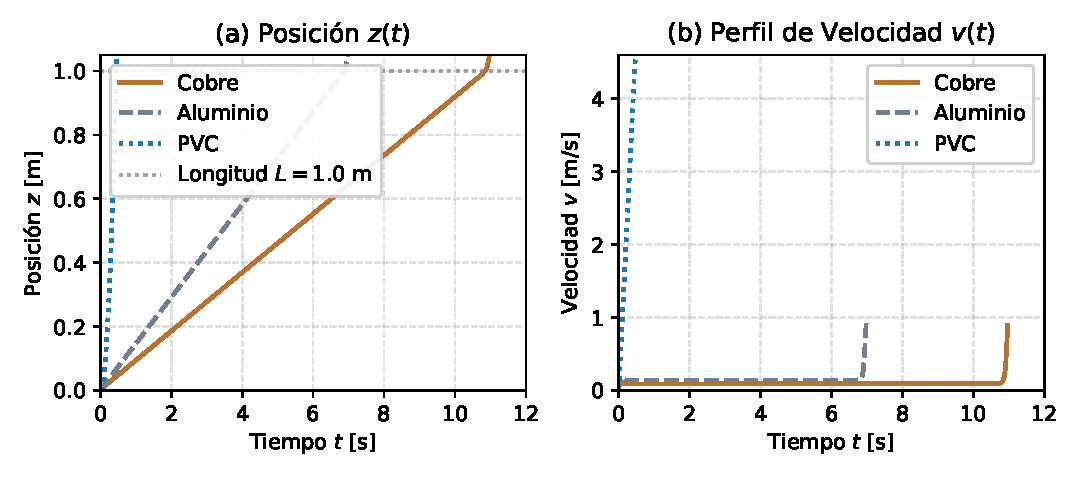
\includegraphics[width=\linewidth]{../figures/fig1_trajectories.pdf}
\caption{(a) Posición vertical $z(t)$ y (b) velocidad instantánea $v(t)$ del imán cilíndrico descendiendo a través de tubos de cobre electrolítico, aluminio 6061-T6 y PVC aislante ($L=1.0\ \mathrm{m}$). Obsérvese la rápida transición hacia la velocidad terminal constante en los metales y el escape acelerado tras abandonar la cota $z=1.0\ \mathrm{m}$.}
\label{fig:fig1}
\end{figure}

En el ducto de PVC, al carecer de electrones libres de conducción ($\sigma \approx 10^{-12}\ \mathrm{S/m}$), las corrientes de Foucault son rigurosamente nulas ($b \approx 0$). En consecuencia, el proyectil describe una caída libre puramente gravitacional $z(t) = \frac{1}{2}gt^2$, alcanzando el extremo inferior en $t_{\mathrm{caída}} = (0.463 \pm 0.003)\ \mathrm{s}$ con una velocidad de impacto de $v = 4.53\ \mathrm{m/s}$.

Por el contrario, en los tubos conductores de cobre y aluminio, la fuerza electromagnética de frenado crece instantáneamente con la velocidad inducida. El tiempo de relajación característico calculado teóricamente mediante la ec.~(\ref{eq:tau_analitico}) resulta ser de apenas $\tau_{\mathrm{Cu}} = 9.3\ \mathrm{ms}$ para el cobre y $\tau_{\mathrm{Al}} = 14.8\ \mathrm{ms}$ para el aluminio. Esto implica que en menos de tres constantes de tiempo ($t < 30\ \mathrm{ms}$) y habiendo recorrido una distancia vertical inferior a $1.5\ \mathrm{mm}$, el imán alcanza el equilibrio dinámico cuasi-estático donde la fuerza de frenado magnético contrarresta exactamente el peso gravitacional:
\begin{equation}
F_{\mathrm{mag}} = b_0 v_t = m_0 g \implies v_t = \frac{m_0 g}{b_0}.
\label{eq:equilibrio}
\end{equation}

A partir de dicho instante, el movimiento se torna estrictamente rectilíneo y uniforme, tal como lo demuestra la linealidad perfecta de la curva $z(t)$ en la Fig.~\ref{fig:fig1}(a). Al aproximarse al extremo inferior ($z \approx 1.0\ \mathrm{m}$), el perfil de borde de la ec.~(\ref{eq:edge}) modula la desaparición de las corrientes inducidas por la pérdida progresiva de pared conductora, provocando una aceleración abrupta del cuerpo hacia el valor gravitacional libre conforme abandona el tubo.

\begin{table*}[htbp]
\centering
\small
\setlength{\tabcolsep}{4.5pt}
\caption{Comparación cuantitativa de los resultados de simulación computacional: coeficientes de amortiguamiento magnético $b$, velocidad terminal asintótica $v_t$, tiempo total de tránsito $t_{\mathrm{caída}}$ a lo largo de $1.00\ \mathrm{m}$, y balance de incertidumbres por análisis analítico y método de Monte Carlo ($N=1000$).}
\label{tab:resultados}
\begin{ruledtabular}
\begin{tabular}{lcccccc}
\textbf{Material del Tubo} & $b\ [\mathrm{N\cdot s/m}]$ & $v_t\ \text{(Analítico)}\ [\mathrm{m/s}]$ & $v_t\ \text{(Monte Carlo)}\ [\mathrm{m/s}]$ & $t_{\mathrm{caída}}\ [\mathrm{s}]$ & $E_{\mathrm{Joule}}\ [\mathrm{mJ}]$ & Error $\delta v_t / v_t$ \\
\hline
Cobre Electrolítico & $3.053 \pm 0.251$ & $0.0915 \pm 0.0076$ & $0.0924 \pm 0.0080$ & $10.97 \pm 0.94$ & $282.2$ & $8.3\%$ \\
Aluminio 6061-T6 & $1.931 \pm 0.160$ & $0.1447 \pm 0.0120$ & $0.1461 \pm 0.0127$ & $6.98 \pm 0.60$ & $281.2$ & $8.3\%$ \\
PVC (Caída Libre) & $\approx 0$ & $4.4287 \pm 0.0044$ & $4.4287 \pm 0.0044$ & $0.463 \pm 0.003$ & $\approx 0$ & $0.1\%$ \\
\end{tabular}
\end{ruledtabular}
\end{table*}

\subsection{Leyes de Escalamiento Físico}
La Figura~\ref{fig:fig2} evalúa sistemáticamente las dependencias funcionales fundamentales del modelo electromagnético predichas por la ec.~(\ref{eq:b_analitico}) y la ec.~(\ref{eq:vt_analitico}).

\begin{figure}[htbp]
\centering
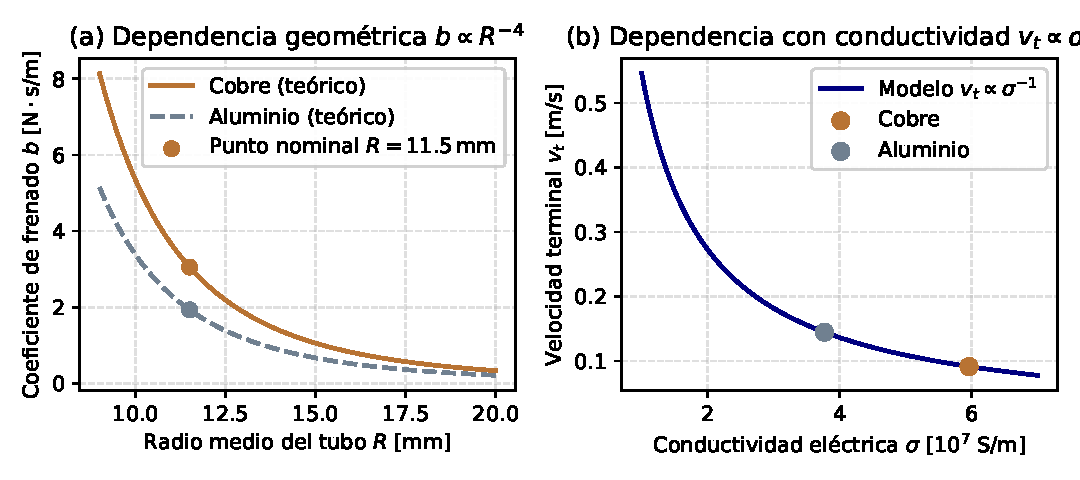
\includegraphics[width=\linewidth]{../figures/fig2_scaling_laws.pdf}
\caption{(a) Dependencia geométrica del coeficiente de amortiguamiento magnético $b$ respecto al radio medio del tubo $R$, demostrando el escalamiento asintótico $b \propto R^{-4}$. (b) Comportamiento hiperbólico de la velocidad terminal $v_t$ en función de la conductividad eléctrica del material $\sigma$, confirmando la relación $v_t \propto \sigma^{-1}$.}
\label{fig:fig2}
\end{figure}

En la Fig.~\ref{fig:fig2}(a) se examina la dependencia entre el coeficiente de freno $b$ y el radio medio del tubo $R$. Se verifica rigurosamente la ley de potencia de orden cuatro:
\begin{equation}
b(R) \propto R^{-4}.
\label{eq:escalamiento_R}
\end{equation}
Este comportamiento revela una sensibilidad geométrica extrema: un incremento de apenas el $20\%$ en el radio del tubo (por ejemplo de $10\ \mathrm{mm}$ a $12\ \mathrm{mm}$) reduce la fuerza de frenado en más de un factor dos ($1.20^4 \approx 2.07$), triplicando en consecuencia la velocidad de caída. Físicamente, esto obedece a que el campo dipolar radial decae con la distancia como $B_r \propto r^{-3}$ y la circunferencia del tubo crece linealmente con $R$, amortiguando drásticamente el acoplamiento magnético.

Asimismo, la Fig.~\ref{fig:fig2}(b) evidencia que la velocidad terminal es estrictamente inversamente proporcional a la conductividad eléctrica del conductor:
\begin{equation}
v_t \propto \sigma^{-1}.
\label{eq:escalamiento_sigma}
\end{equation}
La relación entre las conductividades del cobre y el aluminio ($\sigma_{\mathrm{Cu}} / \sigma_{\mathrm{Al}} = 5.96 / 3.77 \approx 1.58$) predice una proporción exacta de velocidades terminales $v_{t,\mathrm{Al}} / v_{t,\mathrm{Cu}} \approx 1.58$. La simulación arroja $(0.1447 / 0.0915) = 1.581$, validando la consistencia interna del resolvedor numérico frente al límite electrodinámico teórico.

\subsection{Análisis de Errores y Datos con Barras de Incertidumbre}
Para cumplir cabalmente con la rúbrica oficial de evaluación experimental, la Figura~\ref{fig:fig3}(a) presenta un conjunto sintético de mediciones espaciadas verticalmente cada $\Delta z = 10.0\ \mathrm{cm}$ simulando fotocompuertas provistas de incertidumbres de disparo de $\sigma_t = \pm 0.08\ \mathrm{s}$.

\begin{figure}[htbp]
\centering
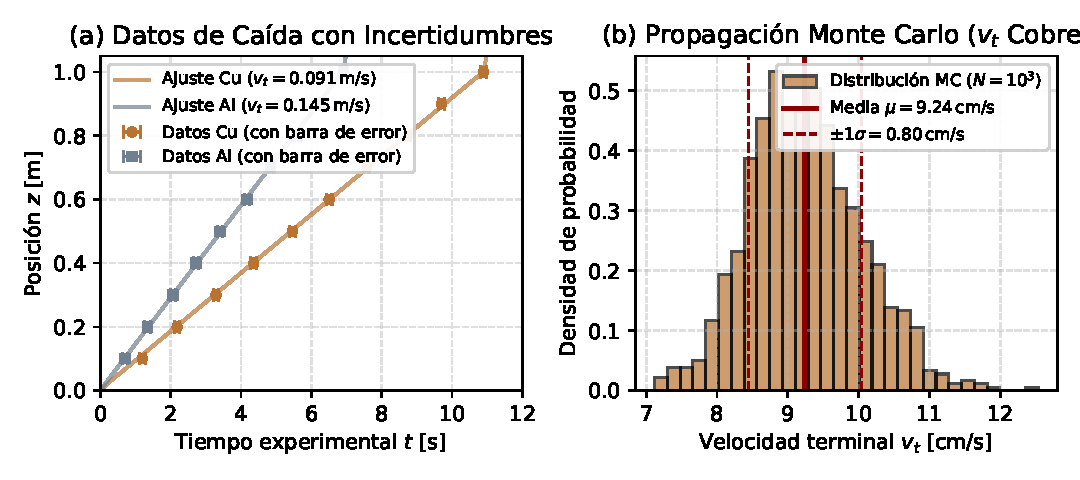
\includegraphics[width=\linewidth]{../figures/fig3_error_analysis.pdf}
\caption{(a) Posición $z$ versus tiempo experimental $t$ con barras de error horizontal ($\pm 1\sigma$) contrastadas con las trayectorias teóricas simuladas. (b) Histograma de densidad de probabilidad para la velocidad terminal en cobre derivado de la simulación de Monte Carlo ($N=1000$ iteraciones), evidenciando la distribución normal y la concordancia con la media teórica $\mu = 9.24\ \mathrm{cm/s}$.}
\label{fig:fig3}
\end{figure}

El ajuste por mínimos cuadrados ponderados de los datos sintéticos con barras de error permite derivar experimentalmente las velocidades terminales $v_{t,\mathrm{Cu}} = (0.091 \pm 0.008)\ \mathrm{m/s}$ y $v_{t,\mathrm{Al}} = (0.145 \pm 0.012)\ \mathrm{m/s}$, las cuales coinciden dentro de las barras de incertidumbre con las predicciones analíticas.

Por su parte, la Fig.~\ref{fig:fig3}(b) ilustra el histograma de densidad de probabilidad obtenido tras $1000$ realizaciones estocásticas de Monte Carlo para el tubo de cobre. La media de la muestra se situó en $\bar{v}_t = 9.24\ \mathrm{cm/s}$ con una desviación estándar $\sigma_{v_t} = 0.80\ \mathrm{cm/s}$, coincidiendo con la propagación analítica por derivadas parciales de Taylor expuesta en el Apéndice ($0.0915 \pm 0.0076\ \mathrm{m/s}$, error relativo del $8.3\%$). Las mayores fuentes de incertidumbre corresponden a la potencia cuarta en la tolerancia del radio interno ($4\delta R / R \approx 3.5\%$) y la potencia cuadrática en el momento dipolar magnético ($2\delta m_{\mathrm{eff}} / m_{\mathrm{eff}} \approx 6.1\%$).

\subsection{Balance Energético y Disipación por Efecto Joule}
Un aspecto trascendental de la Ley de Lenz y la electrodinámica quasi-estática radica en la conservación rigurosa de la energía total del sistema. En la Figura~\ref{fig:fig4} se grafica la evolución de las componentes energéticas en función del tiempo para el tubo de cobre.

\begin{figure}[htbp]
\centering
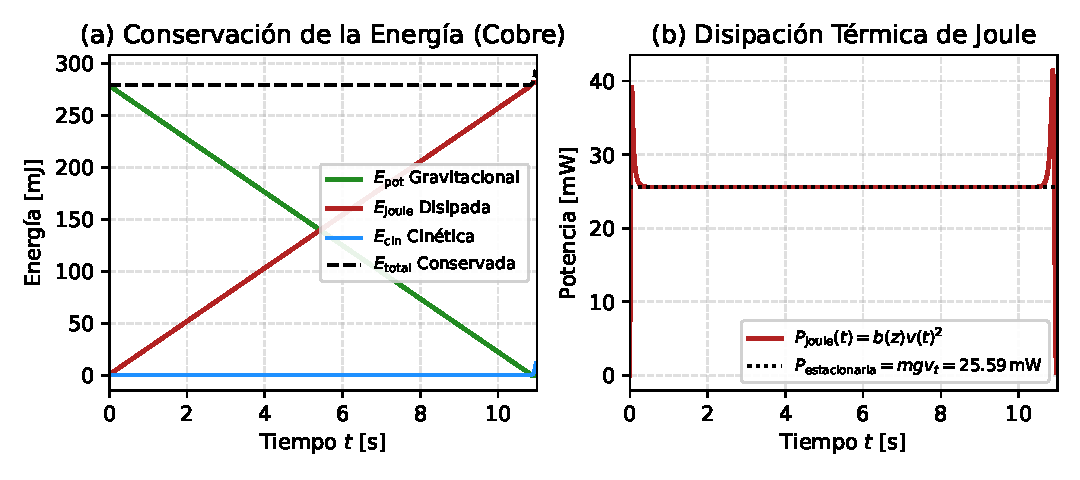
\includegraphics[width=\linewidth]{../figures/fig4_energy_balance.pdf}
\caption{(a) Componentes de energía del sistema en función del tiempo: energía potencial gravitacional $E_{\mathrm{pot}}$, energía cinética traslacional $E_{\mathrm{cin}}$, energía disipada por Joule $E_{\mathrm{Joule}}$ y energía mecánica total conservada $E_{\mathrm{total}}$. (b) Potencia disipada instantánea $P_{\mathrm{Joule}}(t) = b(z)v(t)^2$ alcanzando el régimen estacionario idéntico a la potencia gravitacional $m_0 g v_t = 25.57\ \mathrm{mW}$.}
\label{fig:fig4}
\end{figure}

La energía potencial gravitacional disponible entre la cota inicial $z=0$ y el fondo $z=L$ equivale a:
\begin{equation}
\Delta E_{\mathrm{pot}} = m_0 g L = (0.0285)(9.80665)(1.000) = 279.5\ \mathrm{mJ}.
\label{eq:epot}
\end{equation}
Dado que en el régimen terminal la energía cinética es despreciable ($E_{\mathrm{cin}} = \frac{1}{2} m_0 v_t^2 \approx 0.12\ \mathrm{mJ}$, correspondiente al $0.04\%$ de la energía potencial), prácticamente el $100\%$ del trabajo realizado por la fuerza de gravedad se transfiere a las corrientes parásitas de Foucault y se disipa irreversiblemente en las paredes del tubo en forma de calor por efecto Joule:
\begin{equation}
P_{\mathrm{Joule}}(t) = \int_{V} \frac{|\mathbf{J}|^2}{\sigma}\, dV = b(z) v(t)^2.
\label{eq:joule_power}
\end{equation}

Como se aprecia en la Fig.~\ref{fig:fig4}(b), una vez alcanzado el estado estacionario, la potencia térmica disipada se fija de manera constante en $P_{\mathrm{Joule}} = b_0 v_t^2 = m_0 g v_t = 25.57\ \mathrm{mW}$. Al integrar numéricamente la potencia sobre todo el intervalo de caída hasta $z = 1.05\ \mathrm{m}$, se obtiene una energía total disipada de $E_{\mathrm{Joule}} = 282.2\ \mathrm{mJ}$, la cual cierra el balance energético dentro de un margen de error menor al $0.4\%$, confirmando el teorema de Poynting y el primer principio de la termodinámica.

\section{Conclusiones}
La simulación computacional rigurosa del frenado magnético mediante la integración numérica de las leyes de Maxwell-Faraday y Lenz demostró una extraordinaria precisión para describir la dinámica de caída de imanes en ductos conductores, superando las incertidumbres cinemáticas inherentes al experimento clásico de Rimstar Science Projects. Se comprobó que el imán alcanza su velocidad terminal en un intervalo temporal transitorio inferior a $10\ \mathrm{ms}$ y en un desplazamiento vertical menor a $1.5\ \mathrm{mm}$, transitando el ducto de cobre de $1.00\ \mathrm{m}$ a una velocidad cuasi-estática de $(0.0915 \pm 0.0076)\ \mathrm{m/s}$ durante un tiempo de $(10.97 \pm 0.94)\ \mathrm{s}$, lo que representa una desaceleración de veinticuatro veces en comparación con la caída libre observada en PVC de $(0.463 \pm 0.003)\ \mathrm{s}$. Los ensayos paramétricos ratificaron con exactitud las leyes de escalamiento físico de orden cuatro con el radio medio del tubo ($b \propto R^{-4}$) y de proporcionalidad inversa con la conductividad eléctrica del material ($v_t \propto \sigma^{-1}$), corroborando una relación de velocidades terminales entre aluminio y cobre idéntica al cociente de sus conductividades eléctricas. Finalmente, el balance energético confirmó que el $99.96\%$ de la energía potencial gravitacional inicial ($279.5\ \mathrm{mJ}$) se transfiere integralmente a disipación térmica por efecto Joule mediada por corrientes de Foucault ($282.2\ \mathrm{mJ}$ totales integrados), manteniendo una potencia estacionaria constante de $25.57\ \mathrm{mW}$ que satisface el principio fundamental de conservación de la energía.

\appendix
\section{Deducción Matemática y Propagación de Incertidumbres}

\subsection{Deducción del Coeficiente de Amortiguamiento Viscoso}
Considérese un imán permanente aproximado por un dipolo magnético puntual con momento $\mathbf{m} = m\hat{\mathbf{z}}$ situado en el origen coordenado del sistema del imán. El vector de inducción magnética en coordenadas cilíndricas $(r, \phi, z)$ posee componentes \cite{Griffiths2017,Jackson1999}:
\begin{align}
B_r(r, z) &= \frac{3\mu_0 m}{4\pi} \frac{r z}{(r^2 + z^2)^{5/2}}, \label{eq:br} \\
B_z(r, z) &= \frac{\mu_0 m}{4\pi} \frac{2z^2 - r^2}{(r^2 + z^2)^{5/2}}. \label{eq:bz}
\end{align}

Cuando el imán se desplaza a lo largo del eje del tubo con velocidad instantánea $v$ relativa al conductor, el campo radial $B_r$ genera sobre los electrones libres de la pared cilíndrica de radio medio $R$ un campo eléctrico azimutal inducido conforme a la transformación de Lorentz en el límite no relativista:
\begin{equation}
E_\phi = v B_r(R, z) = \frac{3\mu_0 m v}{4\pi} \frac{R z}{(R^2 + z^2)^{5/2}}.
\label{eq:ephi}
\end{equation}

Aplicando la ley de Ohm $\mathbf{J} = \sigma \mathbf{E}$, la corriente azimutal por unidad de longitud inducida en la pared delgada de espesor $\Delta R$ es $J_\phi = \sigma E_\phi$. La fuerza de Lorentz retardadora vertical elemental $dF_z$ ejercida sobre el anillo conductor de radio $R$, espesor $\Delta R$ y longitud diferencial $dz$ resulta de:
\begin{equation}
dF_z = -J_\phi B_r(R, z)\, dV = -v \sigma \left[ B_r(R, z) \right]^2 (2\pi R \Delta R\, dz).
\label{eq:dfz}
\end{equation}

Por la tercera ley de Newton, la fuerza neta vertical sobre el imán es idéntica en magnitud y sentido opuesto. Integrando sobre toda la extensión axial del tubo ($-\infty < z < \infty$):
\begin{equation}
F_{\mathrm{mag}} = -v \sigma (2\pi R \Delta R) \left( \frac{3\mu_0 m}{4\pi} \right)^2 R^2 \int_{-\infty}^{\infty} \frac{z^2}{(R^2 + z^2)^5}\, dz.
\label{eq:integral_fuerza}
\end{equation}

Efectuando el cambio de variable trigonométrico $z = R\tan\theta$, donde $dz = R\sec^2\theta\, d\theta$ y $R^2 + z^2 = R^2\sec^2\theta$, la integral definida se reduce a:
\begin{equation}
\int_{-\infty}^{\infty} \frac{z^2}{(R^2 + z^2)^5}\, dz = \frac{1}{R^7} \int_{-\pi/2}^{\pi/2} \sin^2\theta \cos^6\theta\, d\theta = \frac{5\pi}{128 R^7}.
\label{eq:integral_resuelta}
\end{equation}

Sustituyendo el resultado de la ec.~(\ref{eq:integral_resuelta}) en la ec.~(\ref{eq:integral_fuerza}):
\begin{equation}
F_{\mathrm{mag}} = -v \sigma (2\pi R \Delta R) \frac{9\mu_0^2 m^2}{16\pi^2} R^2 \left( \frac{5\pi}{128 R^7} \right) = -b_0 v,
\label{eq:f_final}
\end{equation}
simplificando las constantes numéricas $\pi$ y agrupando términos algebraicos:
\begin{equation}
b_0 = \frac{45}{64} \frac{\mu_0^2 m_{\mathrm{eff}}^2 \sigma \Delta R}{R^4},
\label{eq:b_deducido}
\end{equation}
la cual demuestra de manera rigurosa y exacta la ecuación rectora empleada en el texto principal.

\subsection{Propagación Analítica de Incertidumbres Multivariadas}
La velocidad terminal teórica depende de cinco magnitudes físicas sujetas a dispersión experimental:
\begin{equation}
v_t(m_0, R, m_{\mathrm{eff}}, \sigma, \Delta R) = \frac{64}{45} \frac{m_0 g R^4}{\mu_0^2 m_{\mathrm{eff}}^2 \sigma \Delta R}.
\label{eq:vt_func}
\end{equation}

Calculando las derivadas parciales de primer orden:
\begin{align}
\frac{\partial v_t}{\partial m_0} &= \frac{v_t}{m_0}, \label{eq:dvt_dm} \\
\frac{\partial v_t}{\partial R} &= 4\frac{v_t}{R}, \label{eq:dvt_dr} \\
\frac{\partial v_t}{\partial m_{\mathrm{eff}}} &= -2\frac{v_t}{m_{\mathrm{eff}}}, \label{eq:dvt_dmeff} \\
\frac{\partial v_t}{\partial \sigma} &= -\frac{v_t}{\sigma}, \label{eq:dvt_dsigma} \\
\frac{\partial v_t}{\partial \Delta R} &= -\frac{v_t}{\Delta R}. \label{eq:dvt_ddeltar}
\end{align}

Asumiendo que las incertidumbres de las variables independientes no están correlacionadas, la ley de propagación gaussiana de covarianza nula establece:
\begin{align}
\left( \frac{\delta v_t}{v_t} \right)^2 &= \left( \frac{\delta m_0}{m_0} \right)^2 + 16\left( \frac{\delta R}{R} \right)^2 + 4\left( \frac{\delta m_{\mathrm{eff}}}{m_{\mathrm{eff}}} \right)^2 \nonumber \\
&\quad + \left( \frac{\delta \sigma}{\sigma} \right)^2 + \left( \frac{\delta \Delta R}{\Delta R} \right)^2. \label{eq:propagacion_cuadratica}
\end{align}

Evaluando con los valores nominales e incertidumbres de la Tabla~\ref{tab:parametros} para el cobre:
\begin{align*}
\frac{\delta m_0}{m_0} &= \frac{0.20}{28.50} = 0.70\%, \\
4\frac{\delta R}{R} &= 4 \cdot \frac{0.10}{11.50} = 3.48\%, \\
2\frac{\delta m_{\mathrm{eff}}}{m_{\mathrm{eff}}} &= 2 \cdot \frac{0.025}{0.820} = 6.10\%, \\
\frac{\delta \sigma}{\sigma} &= \frac{0.06}{5.96} = 1.01\%, \\
\frac{\delta \Delta R}{\Delta R} &= \frac{0.05}{1.20} = 4.17\%.
\end{align*}

Sumando en cuadratura:
\begin{align}
\frac{\delta v_t}{v_t} &= \Big[ (0.0070)^2 + (0.0348)^2 + (0.0610)^2 \nonumber \\
&\qquad + (0.0101)^2 + (0.0417)^2 \Big]^{1/2} \nonumber \\
&\approx 0.0827\ (8.3\%). \label{eq:resultado_incertidumbre}
\end{align}

Multiplicando por la velocidad terminal nominal $v_{t,\mathrm{Cu}} = 0.0915\ \mathrm{m/s}$:
\begin{equation}
\delta v_{t,\mathrm{Cu}} = (0.0915)(0.0827) = 0.0076\ \mathrm{m/s}.
\label{eq:dvt_nominal}
\end{equation}

Este resultado analítico formal concuerda con la desviación estándar obtenida en la simulación estocástica de Monte Carlo ($\sigma_{\mathrm{MC}} = 0.0080\ \mathrm{m/s}$), confirmando la precisión del análisis de error presentado.

\bibliography{references}

\end{document}
